\documentclass[aspectratio=169, table]{beamer}

\usepackage{listings}
\usepackage{tikz}
\usetikzlibrary{ fit, shapes.geometric, arrows.meta, positioning}
\usepackage{array}
\usepackage{float}
\usepackage{colortbl} 

\lstdefinestyle{RustStyle}{
	language=Java,
	morekeywords={println, Ok, async, fn, main, use, let, mut},
	basicstyle=\ttfamily\scriptsize,
	keywordstyle=\color{blue},
	commentstyle=\color{gray},
	stringstyle=\color{red},
	breaklines=true,
	showstringspaces=false,
	tabsize=2,
	captionpos=b,
	numbers=left,
	numberstyle=\tiny\color{gray},
	frame=lines,
	backgroundcolor=\color{lightgray!10},
	comment=[l]{//},
	morecomment=[s]{/*}{*/},
	commentstyle=\color{gray}\ttfamily,
	string=[s]{'}{'},
	morestring=[s]{"}{"},
	stringstyle=\color{teal}\ttfamily,
	%	showstringspaces=false
	literate=
	{\{}{{\textcolor{red}{\{}}}1
	{\}}{{\textcolor{red}{\}}}}1
	{:}{{\textcolor{red}{:}}}1
	{=}{{\textcolor{red}{=}}}1
	{.}{{\textcolor{red}{.}}}1
	{]}{{\textcolor{red}{]}}}1
	{[}{{\textcolor{red}{[}}}1
	{\#}{{\textcolor{red}{\#}}}1
	{;}{{\textcolor{red}{;}}}1
	{?}{{\textcolor{red}{?}}}1
	{!}{{\textcolor{red}{!}}}1
}

%\usepackage[beamertheme=./praditatheme]{Pradita}

\usetheme{Pradita}

\lstdefinelanguage{bash} {
	keywords={},
	basicstyle=\ttfamily\small,
	keywordstyle=\color{blue}\bfseries,
	ndkeywords={iex},
	ndkeywordstyle=\color{purple}\bfseries,
	sensitive=true,
	commentstyle=\color{gray},
	stringstyle=\color{red},
	numbers=left,
	numberstyle=\tiny\color{gray},
	breaklines=true,
	frame=lines,
	backgroundcolor=\color{lightgray!10},
	tabsize=2,
	comment=[l]{\#},
	morecomment=[s]{/*}{*/},
	commentstyle=\color{gray}\ttfamily,
	stringstyle=\color{purple}\ttfamily,
	showstringspaces=false
}


\title{\Huge Serverless\\Architecture\\}
\subtitle{IF231303-Software Architecture}
\author{\textbf{Alfa Yohannis}}
\begin{document}
	
	\frame{\titlepage}
	
	
	\begin{frame}[fragile]
		\frametitle{Contents}
		\vspace{20pt}
		\begin{columns}[t]
			\column{0.5\textwidth}
			\tableofcontents[sections={1-5}]
			
			\column{0.5\textwidth}
			\tableofcontents[sections={6-10}]
		\end{columns}
	\end{frame}
	
	
	\section{Pendahuluan}
	
	\begin{frame}[fragile]{Pendahuluan: Serverless Architecture}
		\vspace{10pt}
		\begin{columns}[T]
			\begin{column}{0.6\textwidth}
				\textbf{Apa itu Serverless?}
				\begin{itemize}
					\item Pendekatan tanpa pengelolaan server eksplisit
					\item Infrastruktur dikelola oleh penyedia cloud
					\item Fokus pada logika bisnis, bukan provisioning
					\item Umumnya berbasis Function-as-a-Service (FaaS)
					\item Fungsi dipicu oleh event dan bersifat stateless
				\end{itemize}
				
				\textbf{Contoh Penggunaan}
				\begin{itemize}
					\item Backend API
					\item ETL pipeline
					\item Real-time analytics
					\item Chatbot dan automation task
				\end{itemize}
			\end{column}
			
			\begin{column}{0.4\textwidth}
				\textbf{Keunggulan}
				\begin{itemize}
					\item Hemat biaya: bayar saat fungsi berjalan
					\item Otomatis diskalakan
					\item Ringan dan cepat dikembangkan
				\end{itemize}
				
				\textbf{Tantangan}
				\begin{itemize}
					\item Cold start latency
					\item Waktu eksekusi terbatas
					\item Debugging lebih kompleks
				\end{itemize}
				
				\vspace{4pt}
				\scriptsize
				\textit{Perlu pemahaman menyeluruh sebelum mengadopsinya di produksi.}
			\end{column}
		\end{columns}
	\end{frame}
	
	
	
\section{Contoh Kasus Penggunaan}
	
	\begin{frame}[fragile]{Contoh Kasus Penggunaan Serverless}
		\vspace{6pt}
		\begin{columns}[T]
			\begin{column}{0.5\textwidth}
				\textbf{1. Backend Tanpa Server}
				\begin{itemize}
					\item Menjalankan logika bisnis tanpa kelola server
					\item Fungsi berjalan di cloud sebagai respon event
					\item Terhubung ke API Gateway dan database cloud
					\item Contoh:
					\begin{itemize}
						\item Aplikasi e-commerce: fungsi \texttt{ProcessOrder} pada saat checkout
						\item Validasi data → hitung total → panggil payment service
					\end{itemize}
					\item Skalabilitas otomatis dan biaya berbasis eksekusi
				\end{itemize}
			\end{column}
			
			\begin{column}{0.5\textwidth}
				\textbf{2. Integrasi API dan Event}
				\begin{itemize}
					\item Fungsi serverless dipicu oleh HTTP, DB, storage, atau queue
					\item Contoh:
					\begin{itemize}
						\item Upload file ke storage → proses otomatis (resize, ekstraksi metadata)
						\item Perubahan data inventori → update analitik / kirim notifikasi
					\end{itemize}
					\item Mendukung sistem modular dan event-driven
					\item Meningkatkan otomatisasi dan efisiensi
				\end{itemize}
				
				\vspace{6pt}
				\scriptsize
				\textit{Pendekatan ini cocok untuk sistem dinamis yang responsif dan hemat biaya.}
			\end{column}
		\end{columns}
	\end{frame}
	
	\section{Kelebihan dan Kekurangan}
	
	\begin{frame}[fragile]{Kelebihan dan Kekurangan }
		\vspace{10pt}
		\begin{columns}[T]
			\begin{column}{0.5\textwidth}
				\textbf{Kelebihan}
				\begin{itemize}
					\item \textbf{Tanpa Kelola Server:} Tidak perlu provisioning, patching, atau scaling manual.
					\item \textbf{Bayar per Eksekusi:} Biaya hanya saat fungsi dijalankan.
					\item \textbf{Skalabilitas Otomatis:} Fungsi diskalakan sesuai beban secara horizontal.
					\item \textbf{Cepat Rilis:} Fokus ke logika bisnis, tidak ke infrastruktur.
					\item \textbf{Integrasi Mudah:} Terhubung ke layanan cloud (DB, storage, dsb).
				\end{itemize}
			\end{column}
			
			\begin{column}{0.5\textwidth}
				\textbf{Kekurangan}
				\begin{itemize}
					\item \textbf{Cold Start:} Fungsi jarang dipanggil bisa lambat di awal.
					\item \textbf{Batas Eksekusi:} Ada limit waktu, memori, dan ukuran.
					\item \textbf{Stateless:} Status harus disimpan di luar fungsi.
					\item \textbf{Sulit Debugging:} Observasi runtime perlu alat tambahan.
					\item \textbf{Vendor Lock-in:} Migrasi sulit jika pakai fitur spesifik platform.
				\end{itemize}
				
				\vspace{6pt}
				\scriptsize
				\textit{Pahami kekuatan dan batasan sebelum mengadopsinya.}
			\end{column}
		\end{columns}
	\end{frame}
	
	

	
	\section{Konsep Dasar}
	
	\begin{frame}[fragile]{Konsep Dasar Serverless Architecture}
		\vspace{10pt}
		\begin{columns}[T]
			\begin{column}{0.5\textwidth}
				\textbf{1. Function-as-a-Service (FaaS)} \\
				Kode ringan dijalankan saat event terjadi.
				\begin{itemize}
					\item Fokus satu tugas spesifik
					\item Platform: AWS Lambda, GCP Functions
					\item Cocok untuk API, async task, cron job
				\end{itemize}
				
				\vspace{6pt}
				\textbf{2. Event Trigger \& Eksekusi} \\
				Fungsi dipicu oleh event (HTTP, DB, storage, jadwal).
				\begin{itemize}
					\item Eksekusi otomatis oleh platform
					\item Sumber daya hanya aktif saat dibutuhkan
				\end{itemize}
			\end{column}
			
			\begin{column}{0.5\textwidth}
				\textbf{3. Cold Start \& Skalabilitas} \\
				Cold start = latensi awal fungsi jarang aktif.
				\begin{itemize}
					\item Butuh inisialisasi runtime
					\item Instans hangat kurangi delay
					\item Skalabilitas otomatis dan paralel
				\end{itemize}
				
				\vspace{6pt}
				\textbf{4. Lifecycle \& Statelessness} \\
				Fungsi berjalan singkat dan tidak simpan status.
				\begin{itemize}
					\item Status dikelola di luar (DB, storage)
					\item Mudah diskalakan dan diganti
				\end{itemize}
				
				\vspace{4pt}
				\scriptsize
				\textit{Empat konsep ini menjadi fondasi memahami Serverless.}
			\end{column}
		\end{columns}
	\end{frame}
	



\section{Tipe Arsitektur Serverless}

\begin{frame}[fragile]{Microservice Serverless}
	\vspace{15pt}
	\centering
	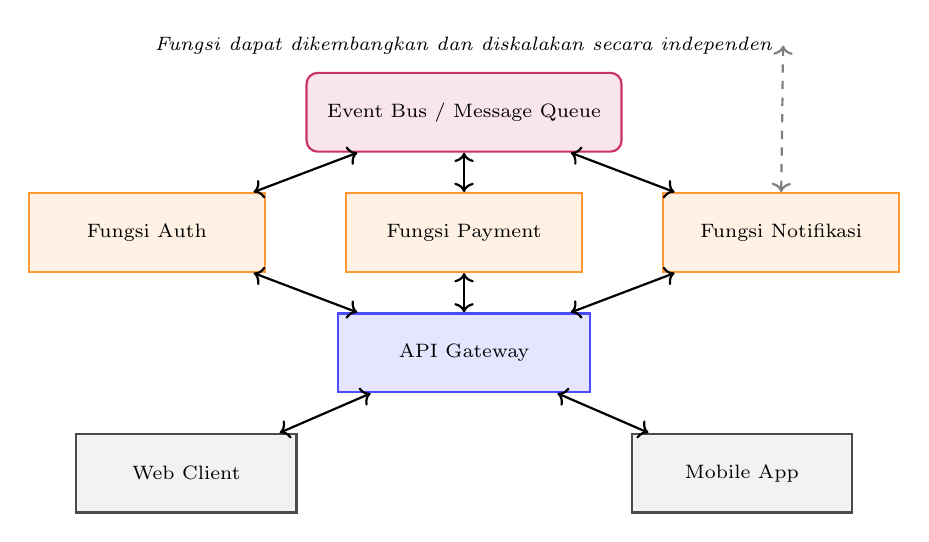
\begin{tikzpicture}[
		node distance=.5cm and 0.5cm,
		every node/.style={font=\scriptsize},
		client/.style={rectangle, draw=black!70, fill=gray!10, thick, minimum width=2.8cm, minimum height=1cm, align=center},
		gateway/.style={rectangle, draw=blue!70, fill=blue!10, thick, minimum width=3.2cm, minimum height=1cm, align=center},
		function/.style={rectangle, draw=orange!80, fill=orange!10, thick, minimum width=3cm, minimum height=1cm, align=center},
		queue/.style={rectangle, draw=purple!80, fill=purple!10, thick, minimum width=4cm, minimum height=1cm, align=center, rounded corners},
		arrow/.style={<->, thick},
		notearrow/.style={<->, thick, dashed, draw=gray}
		]
		
		% Layer 1: Event Bus
		\node[queue] (eventbus) at (0,0) {Event Bus / Message Queue};
		
		% Layer 2: Functions
		\node[function, below left=of eventbus] (auth) {Fungsi Auth};
		\node[function, below=of eventbus] (payment) {Fungsi Payment};
		\node[function, below right=of eventbus] (notif) {Fungsi Notifikasi};
		
		% Layer 3: API Gateway
		\node[gateway, below=0.5cm of payment] (api) {API Gateway};
		
		% Layer 4: Clients
		\node[client, below left=of api] (web) {Web Client};
		\node[client, below right=of api] (mobile) {Mobile App};
		
		% Arrows: Event bus to functions
		\draw[arrow] (eventbus) -- (auth);
		\draw[arrow] (eventbus) -- (payment);
		\draw[arrow] (eventbus) -- (notif);
		
		% Arrows: functions to API
		\draw[arrow] (auth) -- (api);
		\draw[arrow] (payment) -- (api);
		\draw[arrow] (notif) -- (api);
		
		% Arrows: API to clients
		\draw[arrow] (api) -- (web);
		\draw[arrow] (api) -- (mobile);
		
		% Note
		\node[above=0.1cm of eventbus] (note1) {\textit{Fungsi dapat dikembangkan dan diskalakan secara independen}};
		\draw[notearrow] (note1.east) -- (notif.north);
		
	\end{tikzpicture}

	\scriptsize
	Fungsi serverless bekerja secara modular, menerima event dari bus dan melayani permintaan melalui API Gateway.
\end{frame}


\begin{frame}[fragile]{Serverless Event Processing}
	\vspace{4pt}
	\centering
	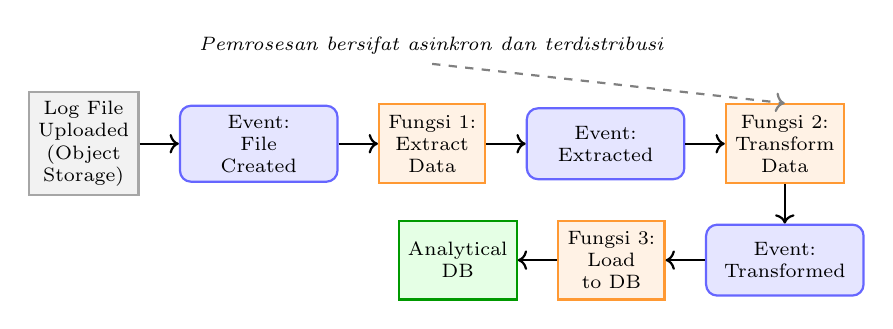
\begin{tikzpicture}[
		node distance=.5cm and .5cm,
		every node/.style={font=\scriptsize},
		source/.style={rectangle, draw=gray!70, fill=gray!10, thick, minimum width=1cm, minimum height=1cm, align=center},
		function/.style={rectangle, draw=orange!80, fill=orange!10, thick, minimum width=1cm, minimum height=1cm, align=center},
		event/.style={rectangle, draw=blue!60, fill=blue!10, thick, rounded corners, minimum width=2cm, minimum height=0.9cm, align=center},
		target/.style={rectangle, draw=green!60!black, fill=green!10, thick, minimum width=1cm, minimum height=1cm, align=center},
		arrow/.style={->, thick},
		notearrow/.style={->, thick, dashed, draw=gray}
		]
		
		% Source: file upload
		\node[source] (storage) {Log File\\Uploaded\\(Object\\Storage)};
		
		% Event 1
		\node[event, right=of storage] (event1) {Event:\\File\\Created};
		
		% Function 1: Extract
		\node[function, right=of event1] (extract) {Fungsi 1:\\Extract\\Data};
		
		% Event 2
		\node[event, right=of extract] (event2) {Event:\\Extracted};
		
		% Function 2: Transform
		\node[function, right=of event2] (transform) {Fungsi 2:\\Transform\\Data};
		
		% Event 3 below Function 2
		\node[event, below=of transform] (event3) {Event:\\Transformed};
		
		% Function 3: Load left of Event 3
		\node[function, left=of event3] (load) {Fungsi 3:\\Load\\to DB};
		
		% Target: DB left of Function 3
		\node[target, left=of load] (db) {Analytical\\DB};
		
		% Arrows
		\draw[arrow] (storage) -- (event1);
		\draw[arrow] (event1) -- (extract);
		\draw[arrow] (extract) -- (event2);
		\draw[arrow] (event2) -- (transform);
		\draw[arrow] (transform) -- (event3);
		\draw[arrow] (event3) -- (load);
		\draw[arrow] (load) -- (db);
		
		% Note
		\node[above=.5cm of extract, align=center] (note1) {\textit{Pemrosesan bersifat asinkron dan terdistribusi}};
		\draw[notearrow] (note1.south) -- (transform.north);
		
	\end{tikzpicture}
	
	\vspace{8pt}
	\scriptsize
	Pipeline ini memproses data secara bertahap menggunakan fungsi yang dipicu oleh event.
\end{frame}


\begin{frame}[fragile]{Hybrid Serverless Architecture}
	\vspace{10pt}
	\begin{columns}[T]
		\begin{column}{0.5\textwidth}
			\textbf{Konsep Utama}
			\begin{itemize}
				\item Gabungan antara serverless dan sistem tradisional (VM, container).
				\item Komponen utama tetap berjalan di arsitektur konvensional.
				\item Fungsi tambahan dijalankan sebagai FaaS (notifikasi, validasi, batch).
				\item Cocok untuk sistem warisan atau masa transisi ke cloud-native.
			\end{itemize}
		\end{column}
		
		\begin{column}{0.5\textwidth}
			\textbf{Contoh Penerapan}
			\begin{itemize}
				\item Aplikasi utama di Kubernetes (session, stateful service).
				\item Fungsi ringan seperti \texttt{SendEmail()}, \texttt{ValidateInput()} pakai Lambda.
				\item Kompatibel dengan arsitektur monolitik yang bertahap dimodernisasi.
			\end{itemize}
			
			\vspace{6pt}
			\scriptsize
			\textit{Hybrid memungkinkan manfaat serverless tanpa mengganggu kestabilan sistem yang ada.}
		\end{column}
	\end{columns}
\end{frame}

\begin{frame}[fragile]{Pola Implementasi: Backend for Frontend}
	\vspace{20pt}
	\centering
	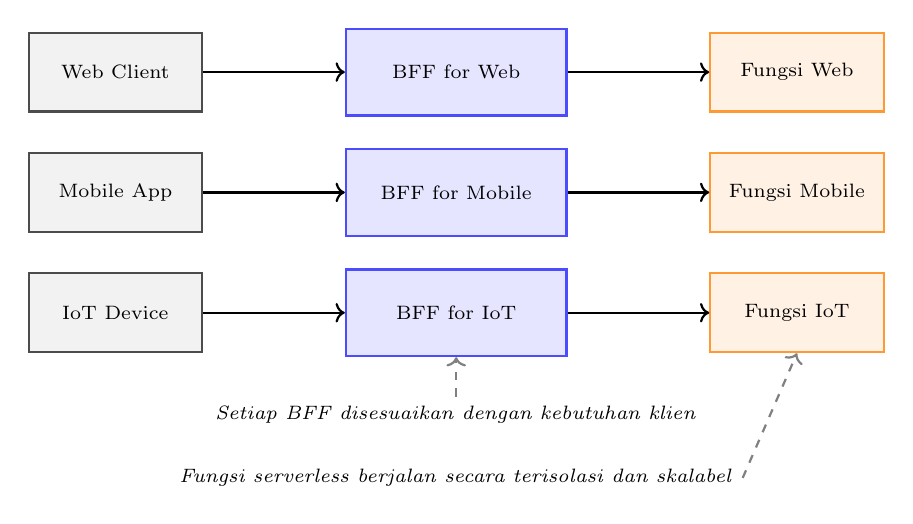
\begin{tikzpicture}[
		node distance=1cm and 1.8cm,
		every node/.style={font=\scriptsize},
		client/.style={rectangle, draw=black!70, fill=gray!10, thick, minimum width=2.2cm, minimum height=1cm, align=center},
		bff/.style={rectangle, draw=blue!70, fill=blue!10, thick, minimum width=2.8cm, minimum height=1.1cm, align=center},
		faas/.style={rectangle, draw=orange!80, fill=orange!10, thick, minimum width=2.2cm, minimum height=1cm, align=center},
		arrow/.style={->, thick},
		notearrow/.style={->, thick, dashed, draw=gray}
		]
		
		% Clients
		\node[client] (web) {Web Client};
		\node[client, below=0.5cm of web] (mobile) {Mobile App};
		\node[client, below=0.5cm of mobile] (iot) {IoT Device};
		
		% BFF Layers
		\node[bff, right=of web] (bff1) {BFF for Web};
		\node[bff, right=of mobile] (bff2) {BFF for Mobile};
		\node[bff, right=of iot] (bff3) {BFF for IoT};
		
		% FaaS layers
		\node[faas, right=of bff1] (faas1) {Fungsi Web};
		\node[faas, right=of bff2] (faas2) {Fungsi Mobile};
		\node[faas, right=of bff3] (faas3) {Fungsi IoT};
		
		% Arrows
		\draw[arrow] (web) -- (bff1);
		\draw[arrow] (mobile) -- (bff2);
		\draw[arrow] (iot) -- (bff3);
		
		\draw[arrow] (bff1) -- (faas1);
		\draw[arrow] (bff2) -- (faas2);
		\draw[arrow] (bff3) -- (faas3);
		
		% Notes
		\node[below=0.5cm of bff3] (note1) {\textit{Setiap BFF disesuaikan dengan kebutuhan klien}};
		\node[below=1.3cm of bff3] (note2) {\textit{Fungsi serverless berjalan secara terisolasi dan skalabel}};
		
		\draw[notearrow] (note1.north) -- (bff3.south);
		\draw[notearrow] (note2.east) -- (faas3.south);
		
	\end{tikzpicture}

	\scriptsize
	Pola BFF memungkinkan setiap jenis klien memiliki backend yang ringan, terisolasi, dan skalabel sesuai kebutuhannya.
\end{frame}


\begin{frame}[fragile]{API Gateway + FaaS}
	\vspace{6pt}
	\centering
	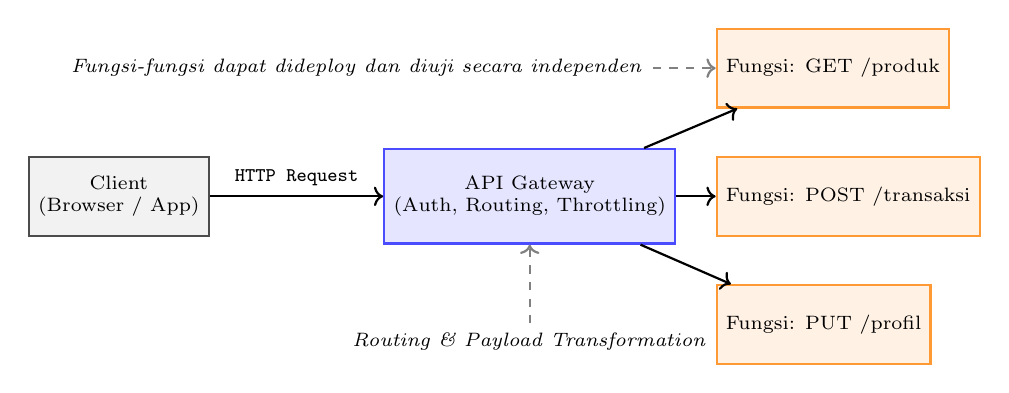
\begin{tikzpicture}[
		node distance=1.5cm and 2.2cm,
		every node/.style={font=\scriptsize},
		client/.style={rectangle, draw=black!70, fill=gray!10, thick, minimum width=2cm, minimum height=1cm, align=center},
		gateway/.style={rectangle, draw=blue!70, fill=blue!10, thick, minimum width=3cm, minimum height=1.2cm, align=center},
		function/.style={rectangle, draw=orange!80, fill=orange!10, thick, minimum width=2.5cm, minimum height=1cm, align=center},
		arrow/.style={->, thick},
		notearrow/.style={->, thick, dashed, draw=gray}
		]
		
		% Nodes
		\node[client] (client) {Client\\(Browser / App)};
		\node[gateway, right=of client] (api) {API Gateway\\(Auth, Routing, Throttling)};
		\node[function, above right=.5cm and .5cm of api] (f1) {Fungsi: GET /produk};
		\node[function, right=.5cm of api] (f2) {Fungsi: POST /transaksi};
		\node[function, below right=.5cm and .5cm of api] (f3) {Fungsi: PUT /profil};
		
		% Arrows
		\draw[arrow] (client) -- node[above] {\texttt{HTTP Request}} (api);
		\draw[arrow] (api) -- (f1);
		\draw[arrow] (api) -- (f2);
		\draw[arrow] (api) -- (f3);
		
		% Notes
		\node[below=1cm of api] (note1) {\textit{Routing \& Payload Transformation}};
		\node[left=0.8cm of f1] (note2) {\textit{Fungsi-fungsi dapat dideploy dan diuji secara independen}};
		
		% Note arrows
		\draw[notearrow] (note1.north) -- (api.south);
		\draw[notearrow] (note2.east) -- (f1.west);
		
	\end{tikzpicture}
	
	\vspace{10pt}
	\scriptsize
	Pola ini memungkinkan klien mengakses fungsi backend secara modular melalui API Gateway yang mengelola otorisasi dan routing.
\end{frame}


\begin{frame}[fragile]{Event-driven Function Chaining}
	\vspace{6pt}
	\centering
	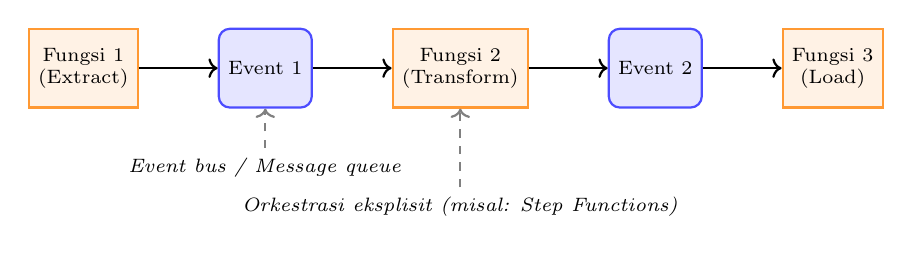
\begin{tikzpicture}[
		node distance=1.5cm and 1cm,
		every node/.style={font=\scriptsize},
		event/.style={rectangle, draw=blue!70, fill=blue!10, thick, rounded corners, minimum width=1cm, minimum height=1cm, align=center},
		function/.style={rectangle, draw=orange!80, fill=orange!10, thick, minimum width=1cm, minimum height=1cm, align=center},
		arrow/.style={->, thick},
		notearrow/.style={->, thick, dashed, draw=gray}
		]
		
		% Nodes
		\node[function] (f1) {Fungsi 1\\(Extract)};
		\node[event, right=of f1] (e1) {Event 1};
		\node[function, right=of e1] (f2) {Fungsi 2\\(Transform)};
		\node[event, right=of f2] (e2) {Event 2};
		\node[function, right=of e2] (f3) {Fungsi 3\\(Load)};
		
		% Arrows
		\draw[arrow] (f1) -- (e1);
		\draw[arrow] (e1) -- (f2);
		\draw[arrow] (f2) -- (e2);
		\draw[arrow] (e2) -- (f3);
		
		% Notes
		\node[below=.5cm of e1] (note1) {\textit{Event bus / Message queue}};
		\node[below=1cm of f2] (note2) {\textit{Orkestrasi eksplisit (misal: Step Functions)}};
		
		% Note arrows
		\draw[notearrow] (note1.north) -- (e1.south);
		\draw[notearrow] (note2.north) -- (f2.south);
		
	\end{tikzpicture}
	
	\vspace{10pt}
	\scriptsize
	Pola ini menyusun fungsi serverless secara berantai berdasarkan alur event untuk membentuk workflow modular.
\end{frame}

\begin{frame}[fragile]{Teknologi Pendukung Serverless Architecture}
	\vspace{20pt}
	\begin{columns}[T]
		\begin{column}{0.33\textwidth}
			\textbf{Cloud Provider Services}
			\begin{itemize}
				\item \textbf{AWS Lambda:} Terintegrasi dengan S3, DynamoDB, API Gateway.
				\item \textbf{Azure Functions:} Cocok untuk Event Grid, Cosmos DB.
				\item \textbf{Google Cloud Functions:} Terhubung ke Pub/Sub, Firestore.
				\item Model event-driven dan autoscaling otomatis.
			\end{itemize}
		\end{column}
		
		\begin{column}{0.33\textwidth}
			\textbf{Infrastructure as Code (IaC)}
			\begin{itemize}
				\item \textbf{Terraform:} Modular, lintas cloud provider.
				\item \textbf{Serverless Framework:} Fokus FaaS, dukung multi-language.
				\item Deployment otomatis, versioning, dan kolaboratif.
				\item Konfigurasi infrastruktur disimpan sebagai kode.
			\end{itemize}
		\end{column}
		
		\begin{column}{0.33\textwidth}
			\textbf{Monitoring \& Observability}
			\begin{itemize}
				\item \textbf{Built-in:} CloudWatch, App Insights, Cloud Monitoring.
				\item \textbf{Eksternal:} Datadog, New Relic, Grafana.
				\item \textbf{Tracing:} AWS X-Ray, OpenTelemetry.
				\item Observasi real-time, debugging, alert otomatis.
			\end{itemize}
			\vspace{4pt}
			\scriptsize
			\textit{Monitoring krusial untuk sistem event-driven yang kompleks.}
		\end{column}
	\end{columns}
\end{frame}




\begin{frame}[fragile]{Best Practices dalam Serverless Architecture}
	\vspace{10pt}
	\begin{columns}[T]
		\begin{column}{0.55\textwidth}
			\textbf{Desain Fungsi}
			\begin{itemize}
				\item Fungsi ringan, fokus satu tugas.
				\item Hindari dependensi besar dan inisialisasi berat.
			\end{itemize}
			
			\textbf{Manajemen State}
			\begin{itemize}
				\item Simpan state di DB, storage, atau cache.
				\item Gunakan event store atau saga untuk koordinasi.
			\end{itemize}
			
			\textbf{Error Handling}
			\begin{itemize}
				\item Bedakan error sementara vs permanen.
				\item Retry pakai backoff; fungsi idempotent.
				\item Kirim gagal ke Dead Letter Queue (DLQ).
			\end{itemize}
		\end{column}
		
		\begin{column}{0.45\textwidth}
			\textbf{Security \& IAM}
			\begin{itemize}
				\item Gunakan prinsip least privilege.
				\item Role/akun terpisah tiap fungsi.
				\item Data terenkripsi dan komunikasi aman.
			\end{itemize}
			
			\textbf{Observability}
			\begin{itemize}
				\item Logging ID, status, dan error.
				\item Kumpulkan metrik dan tracing antar fungsi.
				\item Gunakan alat observasi real-time.
			\end{itemize}
			
			\vspace{6pt}
			\scriptsize
			\textit{Praktik terbaik menjaga sistem tetap efisien, aman, dan mudah ditelusuri.}
		\end{column}
	\end{columns}
\end{frame}

\begin{frame}[fragile]{Implementasi Function-aS AWS Lambda}
	\vspace{10pt}
	Tutorial penggunaan AWS Lambda dan source code-nya dapat diakses melalui:
	
	\vspace{10pt}
	\textbf{Video YouTube:}\\
	\url{https://www.youtube.com/watch?v=kaiB18nG3kc}
	
	\vspace{10pt}
	\textbf{Repository GitHub:}\\
	\url{https://github.com/alfa-yohannis/software-architecture/tree/main/code/chapter12}
	
	\vspace{10pt}
	\scriptsize
	\textit{Contoh ini menunjukkan bagaimana membuat dan menjalankan fungsi sederhana di AWS Lambda untuk memahami prinsip dasar serverless.}
\end{frame}

\begin{frame}[fragile]{Kesimpulan}
	\vspace{10pt}
	\begin{itemize}
		\item \textbf{Serverless Architecture} menghilangkan kebutuhan pengelolaan server dengan mengandalkan layanan cloud berbasis FaaS.
		\item Sistem dibangun secara modular, stateless, dan event-driven dengan skalabilitas otomatis.
		\item Berbagai pola implementasi seperti \textit{BFF}, \textit{API Gateway + FaaS}, dan \textit{Function Chaining} mendukung fleksibilitas desain.
		\item Tantangan mencakup cold start, debugging, manajemen state, dan observabilitas.
		\item Praktik terbaik seperti fungsi ringan, IAM ketat, retry strategy, dan monitoring yang baik menjadi kunci keberhasilan.
		\item Dengan pemahaman menyeluruh dan alat pendukung yang tepat, serverless menjadi fondasi solusi digital yang modern, efisien, dan adaptif.
	\end{itemize}
\end{frame}


\end{document}
